\documentclass{lehramt-informatik}
\InformatikPakete{syntax,er,rmodell}
\usepackage{soul}

\begin{document}

%%%%%%%%%%%%%%%%%%%%%%%%%%%%%%%%%%%%%%%%%%%%%%%%%%%%%%%%%%%%%%%%%%%%%%%%
% Theorie-Teil
%%%%%%%%%%%%%%%%%%%%%%%%%%%%%%%%%%%%%%%%%%%%%%%%%%%%%%%%%%%%%%%%%%%%%%%%

\chapter{Entity-Relation-System}

\begin{quellen}
\item \cite{wiki:entity-relationship-modell}
\end{quellen}

\begin{itemize}
\item Datenmodell: Eignung zur Darstellung des konzeptuellen
Datenbankschemas
\item standardisierte graphische Notation: ER-Diagramm
\item Vorgang der Modellierung: ER-Entwurf
\item Resultat: ER-Modell
\item Vorteil: Kann leicht in Tabellen einer relationalen Datenbank
überführt werden
\item jedoch: nur Strukture der Daten, keine Datenmanipulation
\end{itemize}

\subsection{Begriffsklärung}

Miniwelt:

\begin{itemize}
\item Entity: Object
\item Relationships: Beziehungen zwischen den Werten
\item Attribute: Eigenschaften von Entities oder Relationships
\item Attributewerte: Werte der Attribute
\end{itemize}

Entity-Typen: Gleichartige Entities, mit den gleichen Eigenschaften
Relationship-Typen: Beziehungen gleicher Art

Dabei gilt:

\begin{enumerate}
\def\labelenumi{\arabic{enumi}.}
\item nicht disjunkt: ein Element mehrer Entity-Typen sein.
\item Stelligkeit eines Relationship-Typs
\item Entity-Typ kein mehrere Relationship-Typen haben
\item Schemaebene: Entity-Typ, Relationship-Typ, Attribute; Instanz: Entity,
Relationship, Attributwert
\item Modellierung auf der Schemaebene, keine konkreten Entites
\end{enumerate}

\subsection{Graphische Notation}

\begin{itemize}
\item Entity-Typen: Rechtecke
\item Relationship-Type: Rauten
\item Attribute: Ovale
\end{itemize}

\subsection{Rollennamen}

Zur genaueren Charakterisierung von Entity-Typen und Relationship-Typen

\subsection{Domäne}

zulässige Attributewerte

\begin{itemize}
\item extensional: Aufzählung alles zulässigen Werte
\item intensional: Angabe allgemein bekannter Mengen
\end{itemize}

Mehrwertiges Attribute (Doppelkreis): mehrere Telefonnummern
Abgeleitetes Attribute (gestrichelte Linie): Alter (vom Geburstag)

Relationshiptypen:

\begin{itemize}
\item Binäre zwischen 2 Entitytypen
\item Ternäre zwischen 3 Entitytypten
\end{itemize}

\section{Entity-Relation-System}

% https://usehardware.de/datenbanksysteme-iv-entity-relationship-modell-er-modell-datenbankdarstellungen-i/
\begin{tabular}{cl}

\begin{tikzpicture}
\node[entity] {Entität};
\end{tikzpicture} &
Entität
\\

\begin{tikzpicture}
\node[weak entity] {Entität};
\end{tikzpicture} &
schwache Entität
\\

\begin{tikzpicture}
\node[relationship] {Beziehung};
\end{tikzpicture} &
Beziehung / Relationship
\\

\begin{tikzpicture}
\node[attribute] {Attribut};
\end{tikzpicture} &
einfaches Attribut
\\

\begin{tikzpicture}[node distance=1.6cm]
\node[attribute] (att1) {Attribut};
\node[attribute] (att2) [above right of=att1] {Attribut} edge (att1);
\node[attribute] (att3) [above left of=att1] {Attribut} edge (att1);
\end{tikzpicture} &
zusammengesetztes Attribut
\\

\begin{tikzpicture}
\node[derived attribute] {Attribut};
\end{tikzpicture} &
abgeleitetes Attribut
\\

\begin{tikzpicture}
\node[multi attribute] {Attribut};
\end{tikzpicture} &
Mehrfachattribut
\\

\begin{tikzpicture}
\node[attribute] {\key{Attribut}};
\end{tikzpicture} &
Schlüsselattribut
\\

\begin{tikzpicture}
\node[attribute] {\discriminator{Attribut}};
\end{tikzpicture} &
schwaches Schlüsselattribut
\\

\begin{tikzpicture}
\path[link] (0,0) -- (3,0);
\end{tikzpicture} &
partielle Teilnahme
\\

\begin{tikzpicture}
\path[draw,weak] (0,0) -- (3,0);
\end{tikzpicture} &
totale Teilnahme
\\

\end{tabular}

\begin{itemize}
\item Datenmodell: Eignung zur Darstellung des konzeptuellen
Datenbankschemas
\item standardisierte graphische Notation: ER-Diagramm
\item Vorgang der Modellierung: ER-Entwurf
\item Resultat: ER-Modell
\item Vorteil: Kann leicht in Tabellen einer relationalen Datenbank
überführt werden
\item jedoch: nur Strukture der Daten, keine Datenmanipulation
\end{itemize}

\subsection{Begriffsklärung}

Miniwelt:

\begin{description}
\item[Entity:] Objekt

\item[Entity-Typen:] Gleichartige Entities, mit den gleichen
Eigenschaften

\begin{tikzpicture}
\node[entity] (schulklasse) {Schulklasse};
\end{tikzpicture}

\item[Relationships:] Beziehungen zwischen den Werten

\item[Relationship-Typen:] Beziehungen gleicher Art

\begin{tikzpicture}
\node[relationship,align=center] (hatKlassenleitung) {hatKlassen-\\leitungIn};
\end{tikzpicture}

\item[Attributewerte:] Werte der Attribute

\item[Attribute:] Eigenschaften von Entities oder Relationships

\begin{tikzpicture}
\node[attribute] (klassenzimmer) {Klassenzimmer};
\end{tikzpicture}
\end{description}

Dabei gilt:

\begin{enumerate}
\def\labelenumi{\arabic{enumi}.}
\item nicht disjunkt: ein Element mehrer Entity-Typen sein.
\item Stelligkeit eines Relationship-Typs
\item Entity-Typ kann mehrere Relationship-Typen haben
\item Schemaebene: Entity-Typ, Relationship-Typ, Attribute; Instanz: Entity,
Relationship, Attributwert
\item Modellierung auf der Schemaebene, keine konkreten Entites
\end{enumerate}

\subsection{Rollennamen}

Zur genaueren Charakterisierung von Entity-Typen und Relationship-Typen

\subsection{Domäne}

zulässige Attributewerte

\begin{itemize}
\item extensional: Aufzählung alles zulässigen Werte
\item intensional: Angabe allgemein bekannter Mengen
\end{itemize}

Mehrwertiges Attribut (Doppelkreis): mehrere Telefonnummern
Abgeleitetes Attribut (gestrichelte Linie): Alter (vom Geburstag)

Relationshiptypen:

\begin{itemize}
\item Binäre zwischen 2 Entitytypen
\item Ternäre zwischen 3 Entitytypten
\end{itemize}

%-----------------------------------------------------------------------
%
%-----------------------------------------------------------------------

\section{Generalisierung\footcite[Seite 27]{db:fs:1}}

Die Generalisierung ist eine \memph{Abstraktion auf Ebene der
Entitytypen}, um eine bessere Strukturierung zu erzielen.
%
Die \memph{Eigenschaften ähnlicher Entitytypen} werden einem
\memph{gemeinsamen Obertyp} zugeordnet. Die Eigenschaften (Attribute),
die nicht von den generalisierten Entitytypen geteilt werden, verbleiben
in den Untertypen. Der \memph{Untertyp stellt somit Spezialisierung} des
Obertyps dar.
%
Der \memph{Untertyp erbt alle Eigenschaften} des Obertyps. Die
Entitymenge des Untertyps ist eine Teilmenge der Entitymenge des
Obertyps.
%
Man spricht von einer \memph{disjunkten Spezialisierung}, wenn eine
Entity nur Mitglied von einer der Untertypen ist und es keine
Überschneidungen gibt.
%
\memph{Vollständige Spezialisierung} nennt man die Modellierung, wenn es
keine direkten Elemente des Obertyps gibt. Alle Entitys, die zur Menge
des Obertyps gehören, gehören auch zu einem Untertyp. Der Obertyp ist
Vereinigung der Untertypen.
% https://www.geeksforgeeks.org/generalization-specialization-and-aggregation-in-er-model/
Gezeichnet wird die Generalisierung meist durch ein \memph{Dreieck}.
In manchen Diagrammen stellt ein nach \memph{oben} zeigendes Dreieck die
\memph{Generalisierung}, ein nach unten gerichtetes Dreieick die
\memph{Spezialisierung} dar.

\begin{center}
\begin{tikzpicture}[node distance=1.5cm]
\node[entity] (Person) {Person};
\node[isa,below=of Person] (ISA) {ISA} edge (Person);
\node[entity,below left=of ISA] {Lehrer} edge (ISA);
\node[entity,below right=of ISA] {Schüler} edge (ISA);
\end{tikzpicture}
\end{center}

%-----------------------------------------------------------------------
%
%-----------------------------------------------------------------------

\section{Schwache Entitytypen}

Ein schwacher Entitytypen ist ein Entitytyp, der in seiner Existenz von
einem \memph{anderen Entitytyp abhängig} ist und oft \memph{nur in
Kombination} mit dem Schlüssel des \memph{übergeordneten Entitytyps}
eindeutig identifiziert werden kann.

Eine \memph{Totale Teilnahme} (auch \emph{totale Partizipation} oder
\emph{totale Beteiligung} genannt) liegt dann vor, wenn jede Entität eines
schwachen Entitättypen im Beziehung mit dem übergeordneten Entitytyps steht.

Bespielsweise  kann es keine Entity des Entitytyps \emph{Klassenzimmer}
geben, die keine Beziehung zu einem Entity des Typs \emph{Schulgebäude}
hat. Das bedeutet auch, dass jedes \emph{Schulgebäude} mindestens einen
\emph{Klassenzimmer} hat. Die Nummer eines Klassenzimmers ist nur
innerhalb eines Schulgebäudes eindeutig. Der Schlüssel lautet dann:
\texttt{Klassenzimmers.Nummer} und \texttt{Schulgebäude.Nummer}.

Die Beziehung zwischen \emph{starken} und \emph{schwachem} Typ ist immer
eine \texttt{1:N}-Bezieh\-ung oder \texttt{1:1} in seltenen Fällen.

\footcite[Seite 26]{db:fs:1}

\begin{center}
\begin{tikzpicture}[node distance=1.5cm]
\node[entity] (Schulgebäude) at (0,0) {Schulgebäude};
\node[attribute] (Nummer) [above of=Schulgebäude] {\key{Nummer}} edge (Schulgebäude);
\node[attribute] (Höhe) [below of=Schulgebäude] {Höhe} edge (Schulgebäude);

\node[weak entity] (Klassenzimmer) at (6,0) {Klassenzimmer};
\node[attribute] (Nummer) [above of=Klassenzimmer] {\discriminator{Nummer}} edge (Klassenzimmer);
\node[attribute] (Größe) [below of=Klassenzimmer] {Größe} edge (Klassenzimmer);

\node[ident relationship] (liegtIn) at (3,0) {liegtIn}
  edge (Schulgebäude)
  edge[weak] (Klassenzimmer);
\end{tikzpicture}
\end{center}

%-----------------------------------------------------------------------
%
%-----------------------------------------------------------------------

\section{Funktionalitäten}

Die (min,max)-Notation zählt die Ausprägung von \emph{Beziehungen},
während die anderen Notationen \emph{Entitätstypausprägungen} zählen.
(Wikipedia)

\subsection{einfache / Chen-Notation}

Quellen
\footcite[2.7.1 Seite 41]{kemper}
\footcite[Seite 59]{brinda}

\begin{description}
\item[Schreibweise] 1:1, 1:n, n:1, n:m
\item[Bestimmung]

Auf zu bestimmenden Entitytyp zeigen und Frage formulieren:
%
\emph{„Wie viele X Entities sind in Relationship mit (einem) anderem/n
Entity/ies?“}
%
Das zu bestimmtende Entity ist diesen Fragensätzen \textbf{Objekt}.

\end{description}

\subsection{min-max-Notation / Kardinalitäten}

Quellen
\footcite[2.7.3 Seite 46]{kemper}
\footcite[Seite 62]{brinda}

\begin{description}
\item[Schreibweise] (0, *)
\item[Bestimmung]

Auf zu bestimmenden Entitytyp zeigen und Aussage formulieren:
%
\emph{„Ein Entity ist in Relationship mit X (min, max) anderem/n
Entity/ies“.}
%
Das zu bestimmtende Entity ist diesen Aussagesatz \textbf{Subjekt}.
\end{description}

%%%%%%%%%%%%%%%%%%%%%%%%%%%%%%%%%%%%%%%%%%%%%%%%%%%%%%%%%%%%%%%%%%%%%%%%
% Aufgaben
%%%%%%%%%%%%%%%%%%%%%%%%%%%%%%%%%%%%%%%%%%%%%%%%%%%%%%%%%%%%%%%%%%%%%%%%

\chapter{Aufgaben}

%-----------------------------------------------------------------------
% Zirkus
%-----------------------------------------------------------------------

\section{Zirkus}

\begin{quellen}
\item \cite[Seite 1-2, Aufgabe 1: ER-Diagramm Einstieg]{db:pu:1}
\item \cite[Seite 11, Thema Nr. 2, Aufgabe 2: Relationales Modell]{examen:66116:2018:03}
\item \cite[Seite 6, Aufgabe 2, I. Das Entity-Relationship Modell]{examen:66114:2008:03}
\end{quellen}

Das Fremdenverkehrsamt will sich einen besseren Überblick über Zirkusse
verschaffen. In einer Datenbank sollen dazu die Zirkusse, die
angebotenen Vorstellungen, die einzelnen Darbietungen in einer
Vorstellung sowie die zugehörigen Dompteure und Tiere verwaltet werden.

Ein Zirkus wird durch seinen Namen gekennzeichnet und hat einen
Besitzer. Vorstellungen haben eine \texttt{VorstellungsID} und ein
Datum. Darbietungen haben neben der eindeutigen \texttt{ProgrammNr} eine
Uhrzeit. Ein Dompteur hat eine eindeutige \texttt{AngestelltenNr} sowie
einen Künstlernamen. Tiere sind eindeutig durch eine TierNr bestimmt und
haben außerdem eine Bezeichnung der Tierart.

Ein Zirkus bietet Vorstellungen an und stellt Dompteure an. Eine
Darbietung findet in einer Vorstellung statt. Des weiteren trainiert ein
Dompteur Tiere. In einer Darbietung tritt ein Dompteur mit Tieren auf.

\begin{enumerate}
\item 1.1

\begin{enumerate}

%%
% (a)
%%

\item Listen Sie die Entity-Typen und die zugehörigen Attribute auf.

\begin{minted}{md}
* Zirkusse (Zirkus-Nummer, Namen)
  * Besitzer
  * Namen

* Vorstellungen (VorstellungsID)
  * VorstellungsID
  * Datum

* Darbietungen (ProgrammNr)
  * ProgrammNr
  * Datum

* Dompteuere (AngestelltenNr)
  * AngestelltenNr
  * Künstlernamen

* Tiere (TierNr)
  * TierNr
  * Tierart
\end{minted}

%%
%(b)
%%

\item Bestimmen Sie zu jedem Entity-Typen einen Schlüssel.
Fügen Sie, wenn nötig einen künstlichen Schlüssel hinzu.

\begin{minted}{md}
Zirkus (ZID, Besitzer, Name)
Vorstellung (VorstellungsID, Datum, ZID[Zirkus])
Darbietung (ProgrammNr, VorstellungsID[Vorstellung], Uhrzeit)
Dompteur (AngestelltenNr, Kuenstlername, ZID[Zirkus])
Tier (TierNr, Tierart)

trainiert (AngestelltenNr[Dompteur], TierNr[Tier])
trittAuf (AngestelltenNr[Dompteur], TierNr[Tier], ProgrammNr[Darbietung], VorstellungsID[Vorstellung])
\end{minted}

%%
% (c)
%%

\item Erstellen Sie das ER-Diagramm!

Vorstellungen werden von genau einem Zirkus angeboten. Ein Zirkus bietet
mehrere Vorstellungen an und stellt mehrere Dompteure an. Ein Dompteur
ist genau bei einem Zirkus angestellt. Eine Darbietung findet in einer
bestimmten Vorstellung statt. Des weiteren trainiert ein Dompteur
mehrere Tiere, ein Tier kann allerdings auch von mehreren Dompteuren
trainiert werden. In einer Darbietung tritt genau ein Dompteur mit
mindestens einem Tier auf.
\end{enumerate}

\item 1.2 Ergänzen Sie die Funktionalitäten im ER-Diagramm.

Vorstellungen werden von genau einem Zirkus angeboten. Ein Zirkus bietet
mehrere Vorstellungen an und stellt mehrere Dompteure an. Ein Dompteur
ist genau bei einem Zirkus angestellt. Eine Darbietung findet in einer
bestimmten Vorstellung statt. Des weiteren trainiert ein Dompteur
mehrere Tiere, ein Tier kann allerdings auch von mehreren Dompteuren
trainiert werden. In einer Darbietung tritt genau ein Dompteur mit
mindestens einem Tieren auf.

\item 1.3

\begin{enumerate}

%%
% (a)
%%

\item Was bedeutet „mehrere“?

%%
% (b)
%%

\item Ergänzen Sie die Kardinalitäten in min-max Notation im
ER-Diagramm.

\end{enumerate}

\end{enumerate}

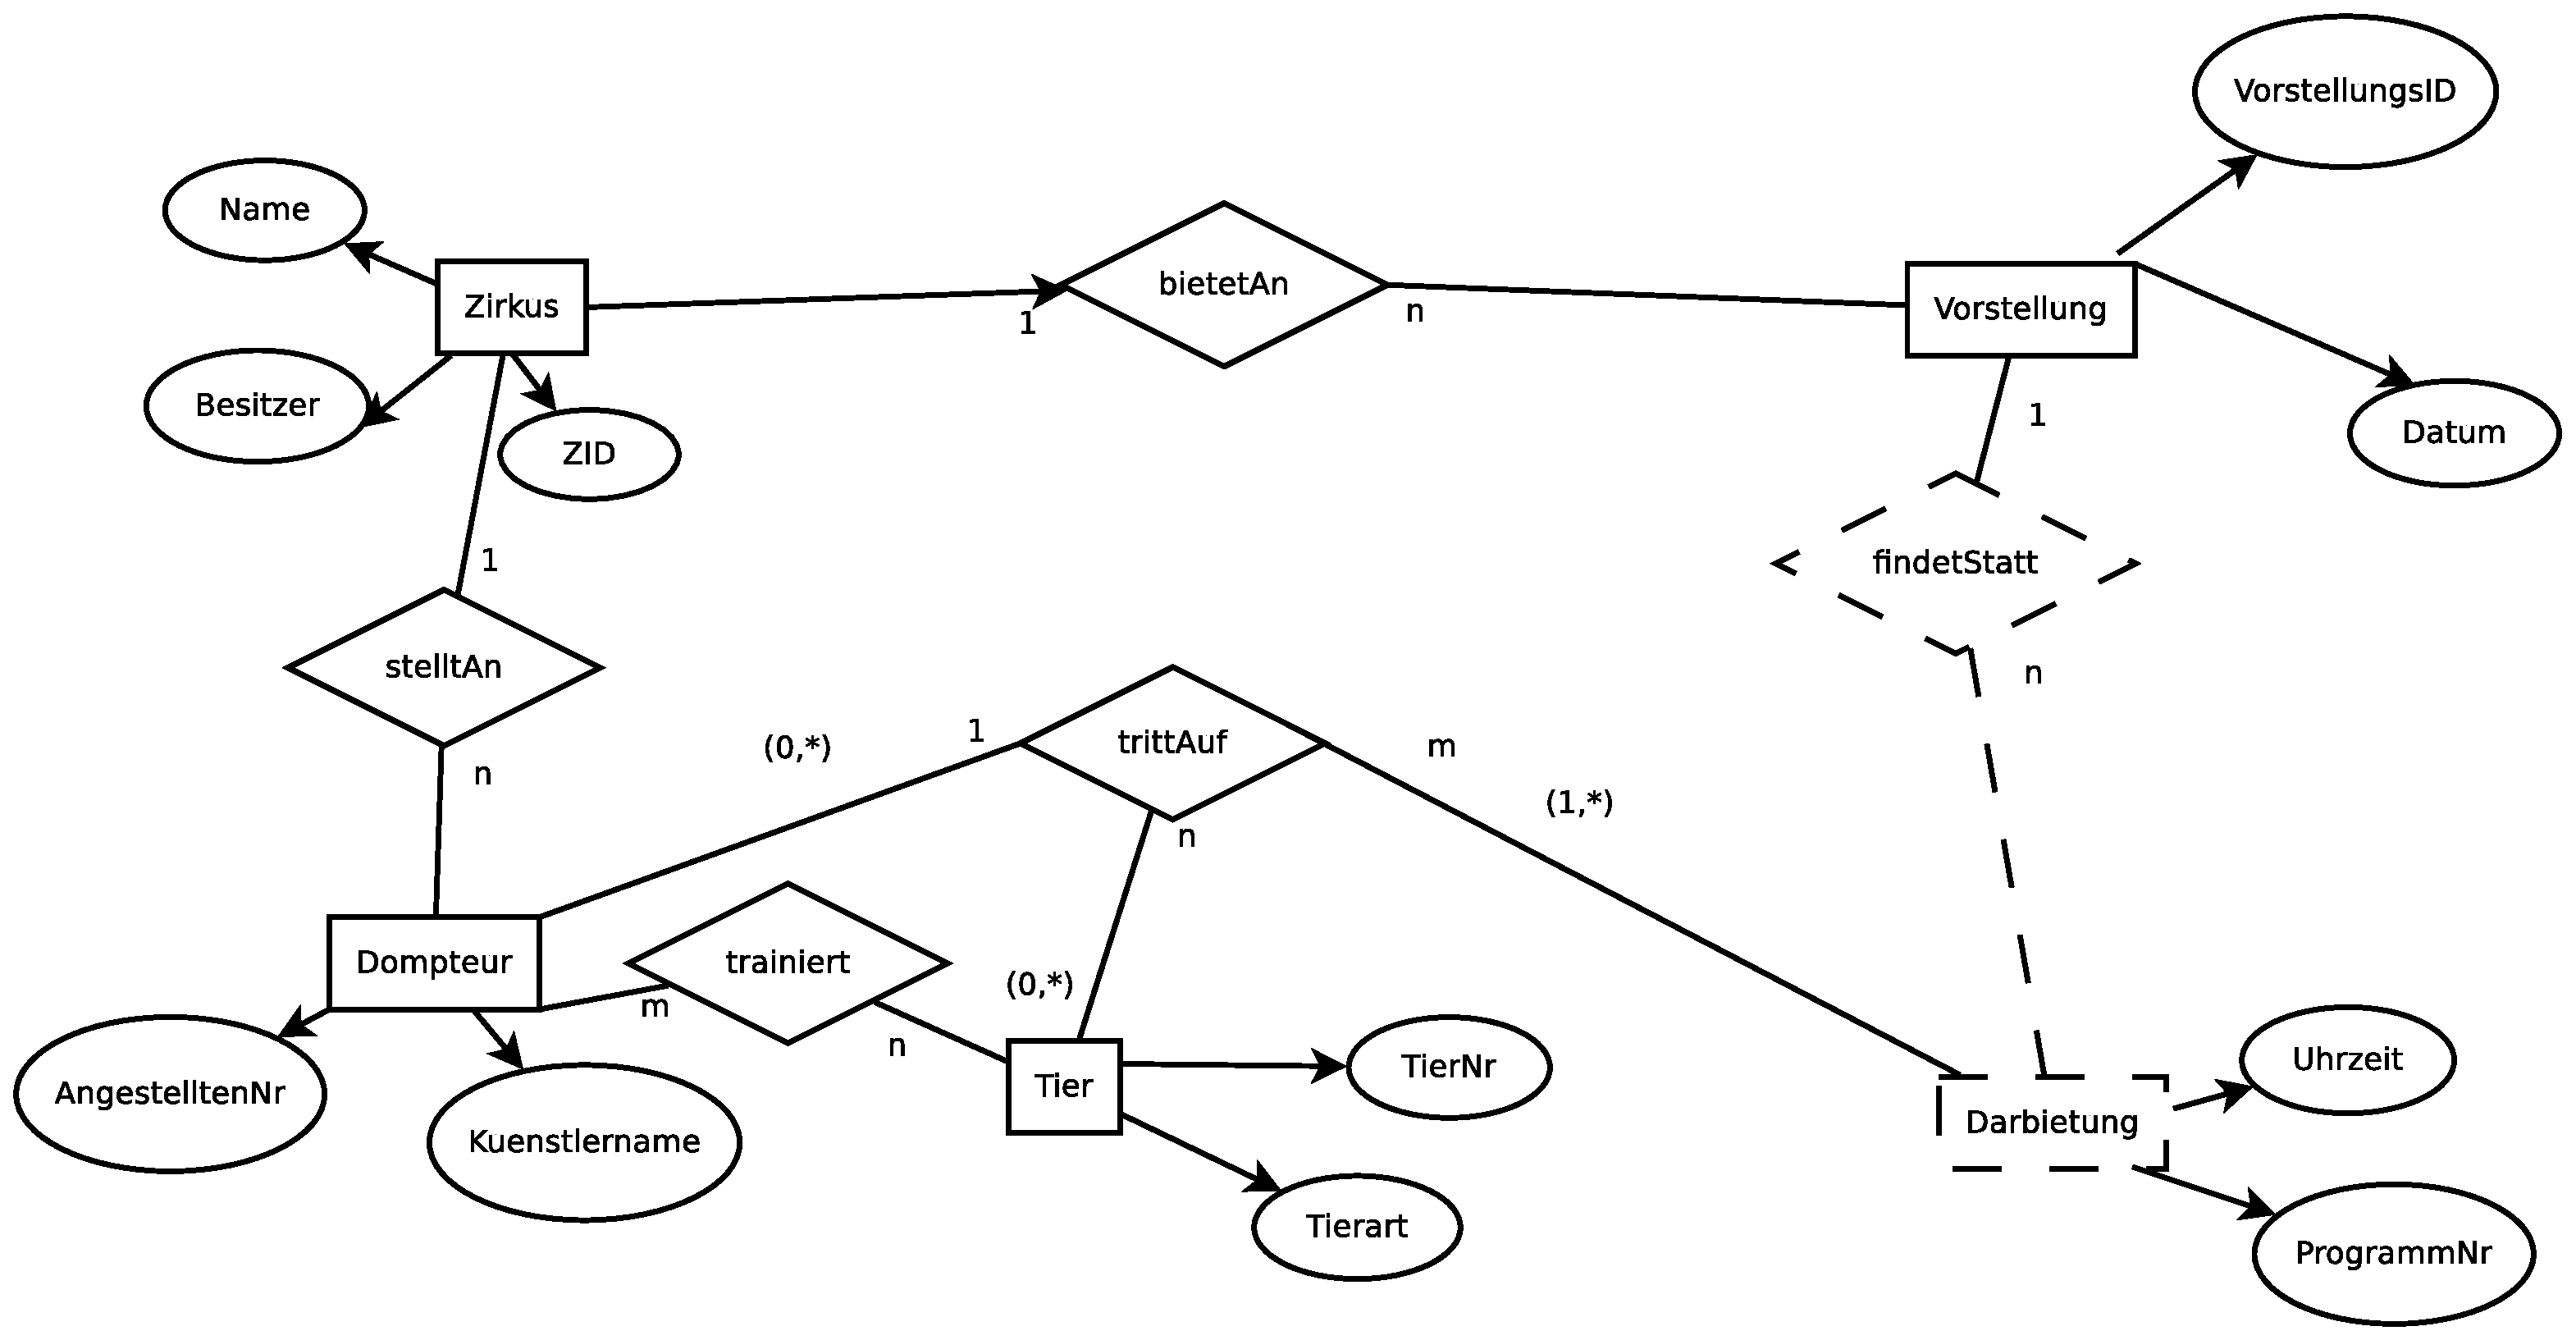
\includegraphics[width=\linewidth]{Zirkus.eps}

%-----------------------------------------------------------------------
% Freizeitparks
%-----------------------------------------------------------------------

\section{Aufgabe 2: ER-Diagramm\footcite[Seite 2]{db:pu:1}}

\noindent
Im Folgenden finden Sie die Beschreibung eines Systems zur Verwaltung
von Freizeitparks. Erstellen Sie zu dieser Beschreibung ein
erweitertes ER-Diagramm. Kennzeichnen Sie die Primär\-schlüssel durch
passendes Unterstreichen und geben Sie die Kardinalitäten in
Chen-Notation (= Funktionalitäten) an. Kennzeichnen Sie auch die totale
Teilnahme (= Existenzabhängigkeit, Partizipität) von Entitytypen.
\footcite[DB/ST - Herbst 2018 (46116, nicht vertieft), Thema 1, TA II, A2]{examen:46116:2018:09}

\begin{itemize}
\item Der \mpEntity{Freizeitpark} ist in mehrere Gebiete
\mpRelationship{eingeteilt}.

\item Ein \mpEntity{Gebiet} hat einen eindeutigen \mpAttribute{Namen}
und eine \mpAttribute{Beschreibung}.

\item In jedem Gebiet \mpRelationship{gibt} es eine oder mehrere
\mpEntity{Attraktionen}. Diese verfügen über eine innerhalb ihres
Gebiets eindeutige \mpAttribute{Nummer}. Außerdem gibt es zu jeder
Attraktion einen \mpAttribute{Namen}, eine \mpAttribute{Beschreibung}
und ein oder mehrere Fotos.

\item Der Freizeitpark \mpRelationship{hat} \mpEntity{Mitarbeiter}. Zu
diesen werden jeweils eine eindeutige \mpAttribute{ID}, der
\mpAttribute{Vorname} und der \mpAttribute{Nachname} gespeichert.
Weiterhin hat jeder Mitarbeiter ein \mpAttribute{Geburtsdatum}, das sich
aus \mpAttribute{Tag}, \mpAttribute{Monat} und \mpAttribute{Jahr}
zusammensetzt.

\item Die Arbeit im Freizeitpark ist in \mpEntity{Schichten}
organisiert. Eine Schicht kann eindeutig durch das \mpAttribute{Datum}
und die \mpAttribute{Startzeit} identifiziert werden. Jede Schicht hat
weiterhin eine \mpAttribute{Dauer}.

\item Mitarbeiter können in Schichten an Attraktionen
\mpRelationship{arbeiten}. Dabei wird die \mpAttribute{Aufgabe}
gespeichert, die der Mitarbeiter übernimmt. Pro Schicht kann der selbe
Mitarbeiter nur an maximal einer Attraktion arbeiten.
\end{itemize}

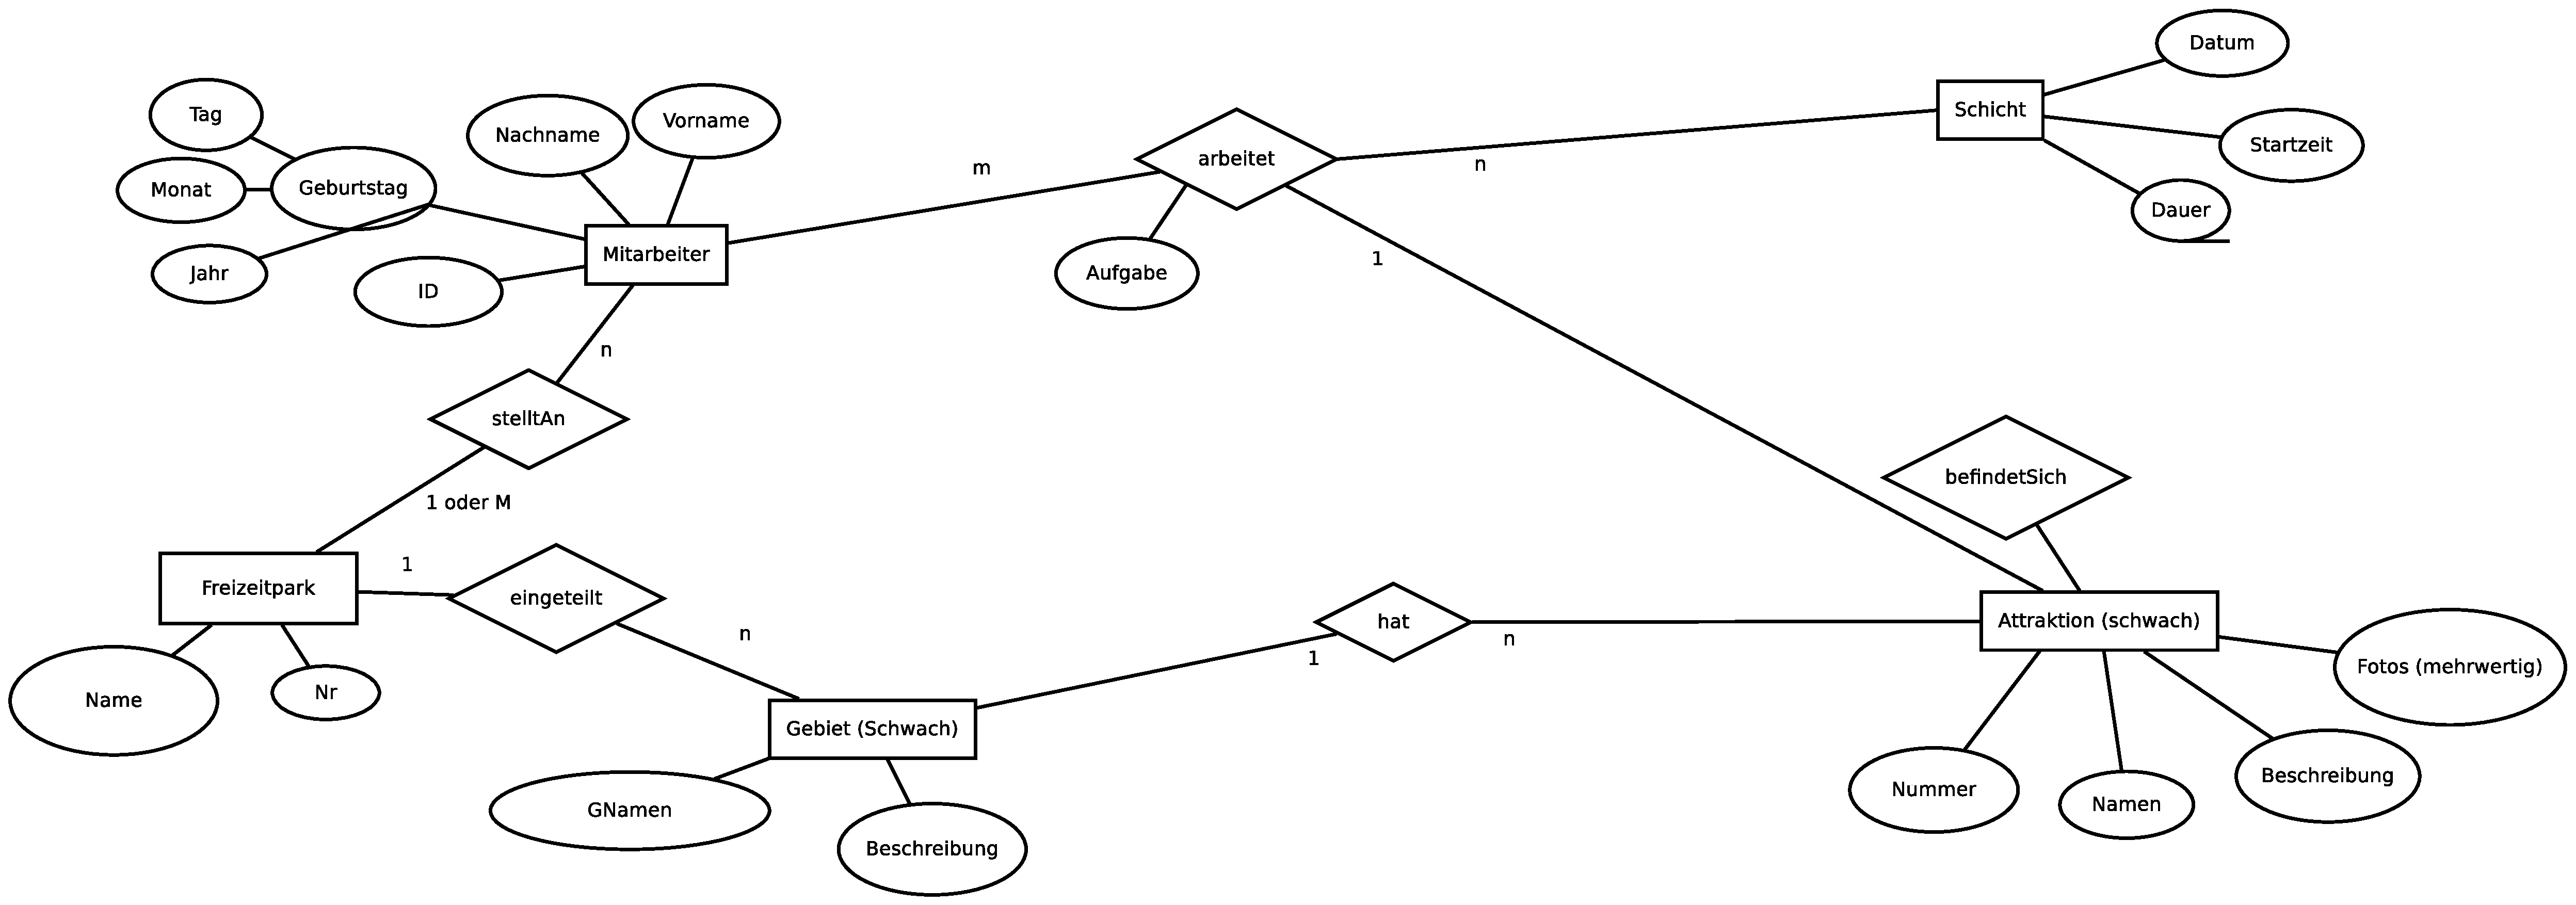
\includegraphics[width=\linewidth]{Freizeitpark.eps}

\begin{tikzpicture}[er2]
\node[entity] (Freizeitpark) {Freizeitpark};

\node[weak entity,right=4cm of Freizeitpark] (Gebiet) {Gebiet};

\node[entity,below=3cm of Freizeitpark] (Mitarbeiter) {Mitarbeiter};

\node[entity,below=3cm of Gebiet] (Schicht) {Schicht};

\node[weak entity,below right=3cm of Mitarbeiter] (Attraktion) {Attraktion};

\end{tikzpicture}

%-----------------------------------------------------------------------
% Mitarbeiter / Abteilung / Projekt
%-----------------------------------------------------------------------

\section{Aufgabe 3: Relationenmodell Einstieg\footcite[Seite 2-3]{db:pu:1}}

\begin{tikzpicture}
\node[entity] (Abteilung) {Abteilung};
\node[attribute,above left=0.5cm and -0.5cm of Abteilung] {\key{AbtID}}
  edge (Abteilung.north);
\node[attribute,above right=0.5cm and -0.5cm of Abteilung] {AName}
  edge (Abteilung.north);

\node[relationship,right=of Abteilung] (gehörtZu) {gehörtZu}
  edge node[auto]{1} (Abteilung);

\node[entity,right=of gehörtZu] (Mitarbeiter) {Mitarbeiter}
  edge node[auto]{n} (gehörtZu);
\node[attribute,above right=0cm and 1cm of Mitarbeiter] {\key{PerID}}
  edge (Mitarbeiter.east);
\node[attribute,below right=0cm and 1cm of Mitarbeiter] {MName}
  edge (Mitarbeiter.east);

\node[relationship,above=1cm of Mitarbeiter] (istChefVon) {istChefVon}
  (istChefVon.east) edge node[auto,pos=0.1]{Untergebener} node[auto,swap,pos=0.4]{n} (Mitarbeiter.north east)
  (istChefVon.west) edge node[auto,swap,pos=0.3]{Chef} node[auto,pos=0.7]{1} (Mitarbeiter.north west);
\node[relationship,below left=1cm and 0cm of Mitarbeiter] (arbeitetMit) {arbeitetMit}
  (arbeitetMit.north) edge node[auto]{m} (Mitarbeiter.south);
\node[relationship,below right=1cm and 0cm of Mitarbeiter] (verantFür) {verantFür}
  (verantFür.north) edge node[auto]{1} (Mitarbeiter.south);

\node[entity,node distance=3cm,below=of Mitarbeiter] (Projekt) {Projekt}
edge node[auto]{n} (arbeitetMit.south) edge node[auto]{1} (verantFür.south);
\node[attribute,above left=-0.25cm and 1cm of Projekt] {\key{ProjID}}
  edge (Projekt.west);
\node[attribute,below left=-0.25cm and 1cm of Projekt] {PName}
  edge (Projekt.west);
\end{tikzpicture}

\begin{enumerate}

%%
% (a)
%%

\item Übertragen Sie das gegebene ER-Modell in ein
relationales Schema! Geben Sie in geeigneter Weise Schlüssel an.

%%
% (b)
%%

\item Verfeinern Sie das Relationenschema!

\begin{antwort}
\begin{minted}{md}
Abteilung (id:AbtId, A_Name)
Mitarbeiter (id:PersID, M_Name, AbtID[Abteilung], Chef[Mitarbeiter])
Projekt (id:ProjID, P_Name, Verantwortlicher (PersId)[Mitarbeiter])
arbeitet_mit (ProjId[Projekt], PersID[Mitarbeiter]) Schlüsselkandiaten: beide
\end{minted}
\end{antwort}

\end{enumerate}

%-----------------------------------------------------------------------
% Zirkus
%-----------------------------------------------------------------------

\section{Aufgabe 4: Relationenmodell}

\begin{enumerate}

%%
% (a)
%%

\item Überführen Sie das ER-Diagramm der Zirkusverwaltung in
ein verfeinertes Relationenschema. Geben Sie die Fremdschlüssel an.

\end{enumerate}

%-----------------------------------------------------------------------
%
%-----------------------------------------------------------------------

\section{Aufgabe 5: ER-Diagramm und Relationenmodell vertieft
\footcite{db:pu:1}}

Sie sollen ein System zur Verwaltung von Pferderennen entwerfen.
Gehen Sie dabei von folgendem Szenario aus:
\footcite[DB/ST - Frühjahr 2013 (46116, nicht vertieft), Thema 1, TA II, A1]{examen:46116:2013:03}

\begin{itemize}
\item \mpEntity{Unternehmen} werden ihre eindeutige
\mpAttribute{Unternehmens-ID} identifiziert. Sie haben eine
\mpAttribute{Adresse} und \mpRelationship{besitzen} Rennställe.

\item Der \mpAttribute{Name} eines \mpEntity{Rennstalls} ist nur
innerhalb eines Unternehmens eindeutig. Für jeden Rennstall wird das
\mpAttribute{Gründungsdatum} gespeichert.

\item \mpEntity{Pferde} \mpRelationship{gehören} immer zu einem
Rennstall. \mpAttribute{Pferdenamen} werden in einem Rennstall nur
jeweils maximal einmal vergeben.

\item \mpEntity{Jockeys} sind in einem Rennstall
\mpRelationship{beschäftigt}. Jeder Rennstall vergibt seine eigenen
\mpAttribute{Personalnummern}. Für jeden Jockey werden
\mpAttribute{Vorname} und \mpAttribute{Name} gespeichert.

\item \mpEntity{Rennen} haben ein \mpAttribute{Datum}, ein
\mpAttribute{Preisgeld} und einen \mpAttribute{Namen}, über den sie
identifiziert werden.

\item Unternehmen \mpRelationship{unterstützen} Rennen finanziell mit
einem bestimmten Betrag.

\item Jockeys \mpRelationship{nehmen} mit Pferden an Rennen teil. Im
Rennen erreichen sie einen bestimmten Platz. Die Kombination aus Jockey
und Pferd ist nicht fest, bei unterschiedlichen Rennen können Jockeys
verschiedene Pferde reiten. Jockeys können auch mit Rennpferden von
fremden Rennställen, die anderen Unternehmen gehören können, an Rennen
teilnehmen.
\end{itemize}

\begin{enumerate}

%%
% (a)
%%

\item Entwerfen Sie für das beschriebene Szenario ein
ER-Modell. Bestimmen Sie hierzu:

\begin{itemize}
\item die Entity-Typen, die Relationship-Typen und jeweils deren
Attribute,

\item ein passendes ER-Diagramm,

\item die Primärschlüssel der Entity-Typen, welche Sie anschließend in
das ER-Diagramm eintragen, und

\item die Funktionalitäten der Relationship-Typen, welche Sie ebenfalls
in das ER-Diagramm eintragen.
\end{itemize}

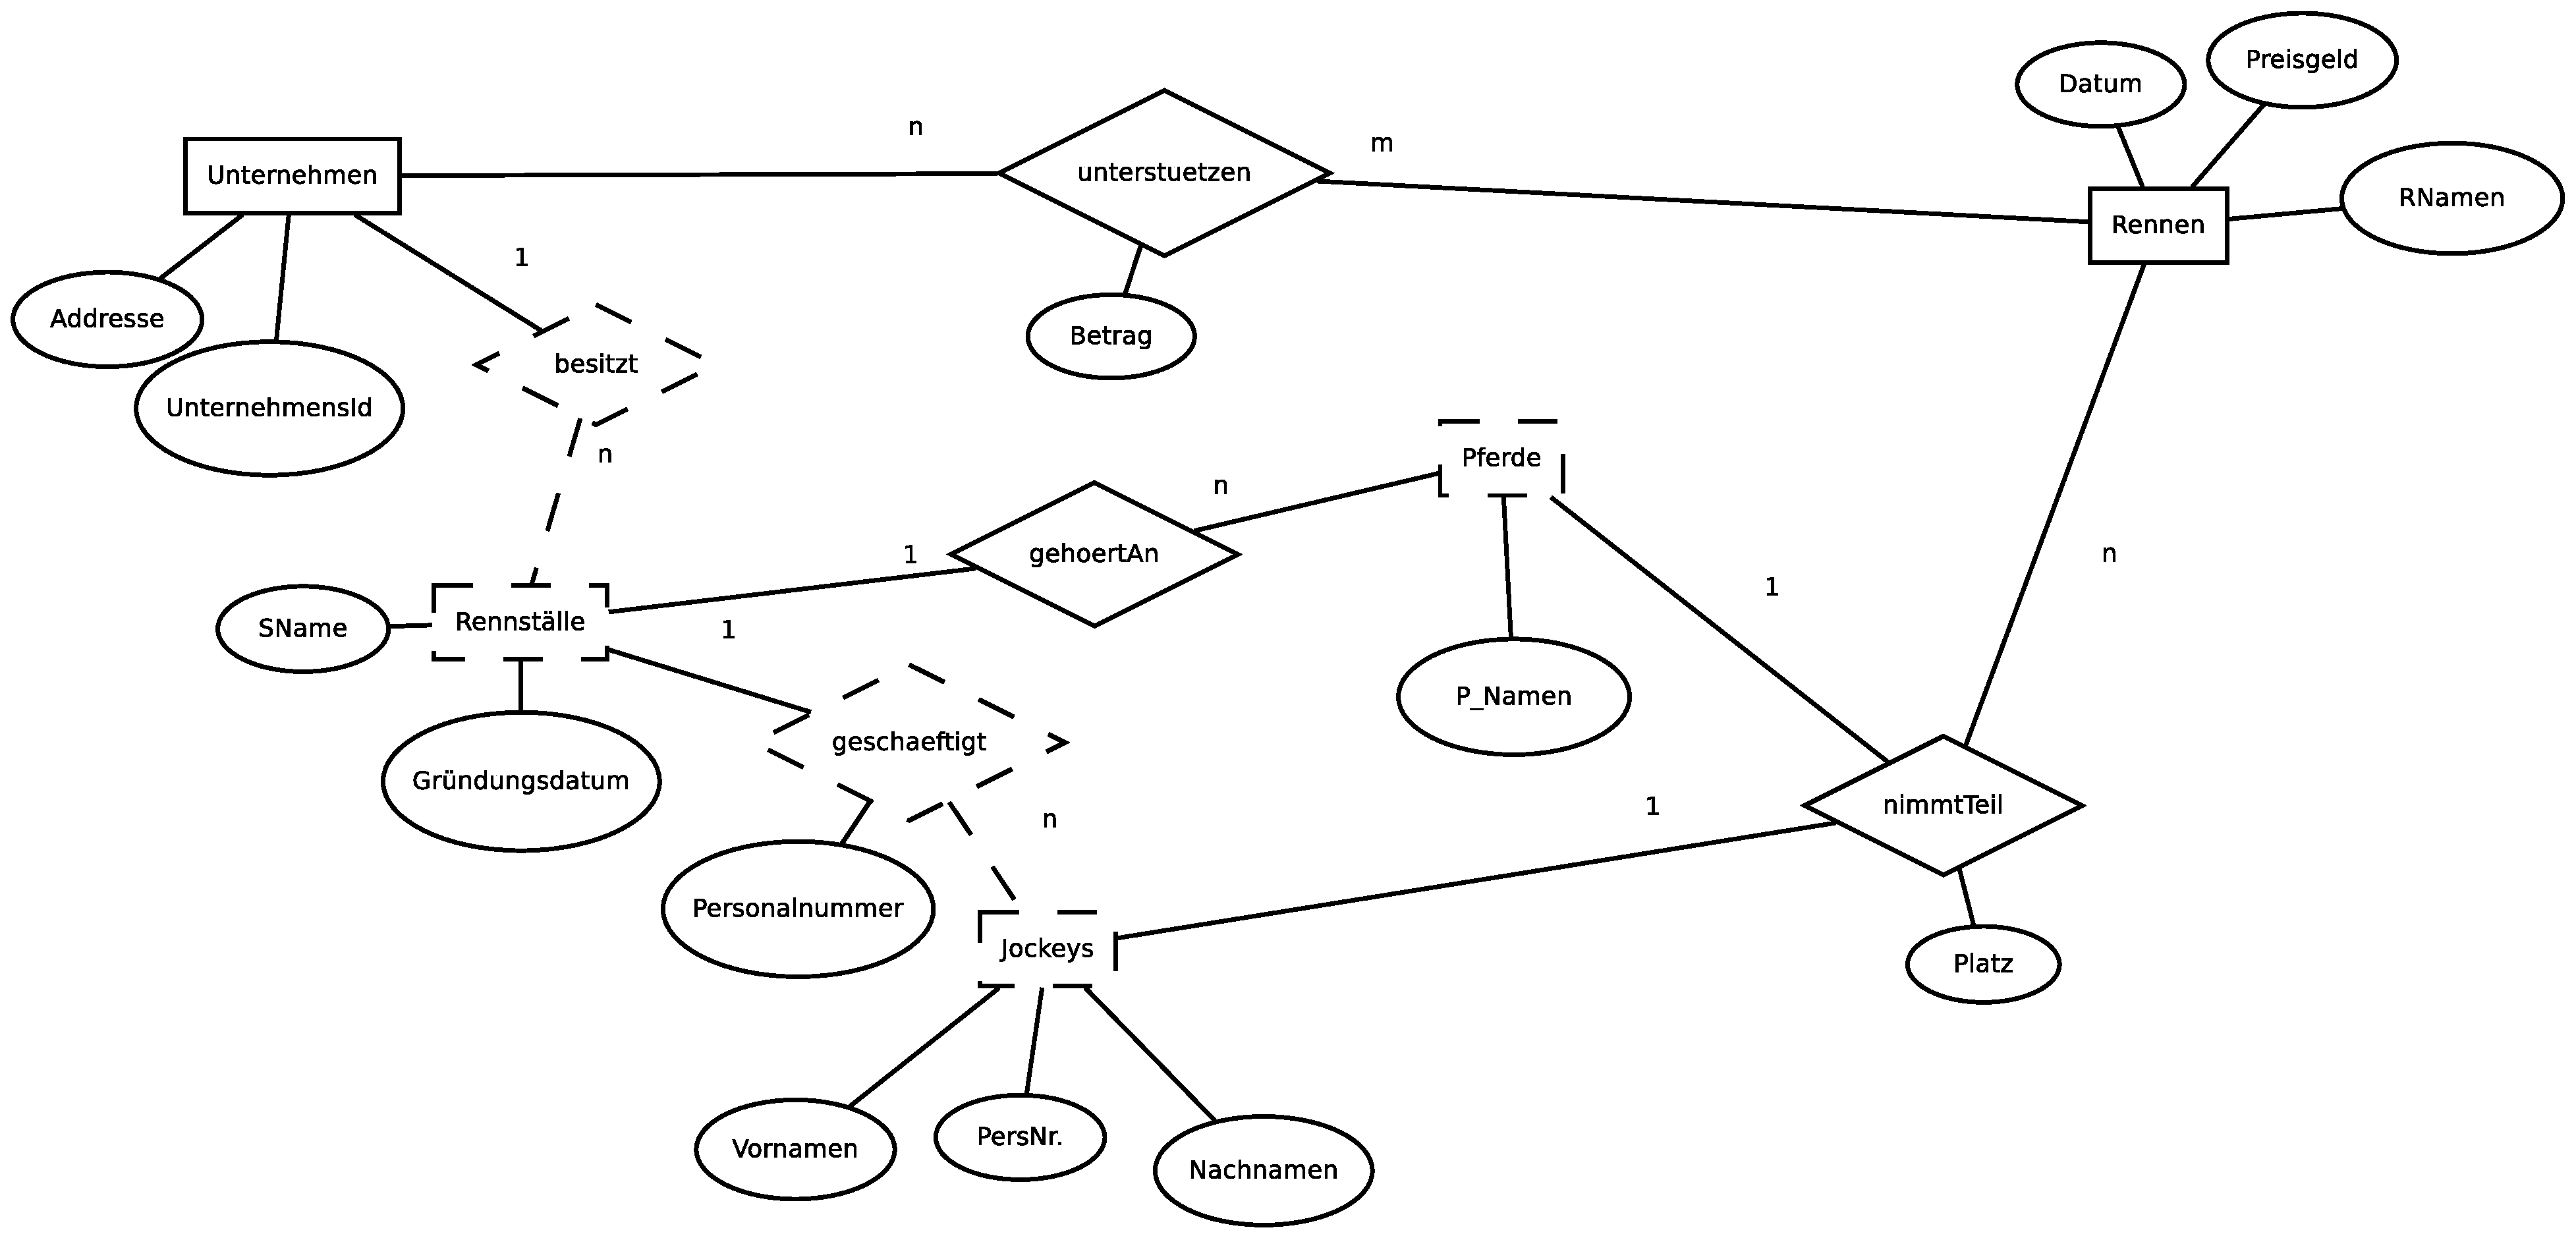
\includegraphics[width=\linewidth]{Rennstaelle.eps}

\begin{antwort}
\begin{center}
\begin{tikzpicture}[er2,scale=0.6,transform shape]
% Unternehmen
\node[entity] (Unternehmen) {Unternehmen};
\node[attribute,above=0.5cm of Unternehmen] (UID) {\key{UID}} edge (Unternehmen);
\node[attribute,left=0.5cm of Unternehmen] (Adresse) {Adresse} edge (Unternehmen);

% Rennstall
\node[weak entity,right=5cm of Unternehmen] (Rennstall) {Rennstall};
\node[attribute,above=0.5cm of Rennstall] (Name) {Name} edge (Rennstall);
\node[attribute,right=0.5cm of Rennstall] (Gründungsdatum) {Gründungsdatum} edge (Rennstall);

% besitzt
\node[ident relationship,right=1.5cm of Unternehmen] (besitzt) {besitzt}
  edge node[auto]{1} (Unternehmen)
  edge[weak] node[auto]{n} (Rennstall);

% Pferd
\node[weak entity,below=4cm of Rennstall] (Pferd) {Pferd};
\node[attribute,right=0.5cm of Pferd] (Name) {\key{Pferdename}}
  edge (Pferd);

% gehören
\node[ident relationship,below=1.5cm of Rennstall] (gehören) {gehören}
  edge node[auto]{1} (Rennstall)
  edge[weak] node[auto]{n} (Pferd);

% Jockey
\node[weak entity,below=4cm of Unternehmen] (Jockey) {Jockey};
\node[attribute,left=0.5cm of Jockey] (Personalnummer) {\key{Personalnummer}}
  edge (Jockey);
\node[attribute,below left=0.5cm of Jockey] (Vorname) {Vorname}
  edge (Jockey);
\node[attribute,below=0.5cm of Jockey] (Name) {Name}
  edge (Jockey);

% beschäftigt
\node[relationship,below=1cm of Unternehmen] (beschäftigt) {beschäftigt}
  edge node[auto]{1} (Unternehmen)
  edge node[auto]{n} (Jockey);

% Rennen
\node[entity,below right=2cm of Jockey] (Rennen) {Rennen};
\node[attribute,below left=0.5cm of Rennen] (Datum) {Datum}
  edge (Rennen);
\node[attribute,below=0.5cm of Rennen] (Preisgeld) {Preisgeld}
  edge (Rennen);
\node[attribute,below right=0.5cm of Rennen] (Name) {Name}
  edge (Rennen);

\node[relationship,right=1cm of Jockey] (teilnehmen) {teilnehmen}
  edge node[auto]{1} (Jockey)
  edge node[auto]{1} (Pferd)
  edge node[auto]{n} (Rennen);
\end{tikzpicture}
\end{center}
\end{antwort}

%%
% (b)
%%

\item Überführen Sie das ER-Modell aus Aufgabe a) in ein verfeinertes
relationales Modell. Geben Sie hierfür die verallgemeinerten
Relationenschemata an. Achten Sie dabei insbesondere darauf, dass die
Relationenschemata keine redundanten Attribute enthalten.

\begin{minted}{md}
Unternehmen (UnternehmensID, Addresse)
Rennstall (S_Name, UnternehmensID[Unternehmen], Gründungsdatum)
Jockey (PersNr, S_Name[Rennstall], ID[Unternehmen], Vorname, Name)
Rennen (R_Name, Datum, Preisgeld)
Pferd (P_Name, S_Namen, UnternehmensID[Unternehmen])

teilnehmen (R_Name[Rennen], PersNr[Jockey], S_Name1, ID1, P_Namen, S_Namen2, ID2, Platz)
unterstuetzen (UnternehmensID[Unternehmen], R_Name[Rennen], Betrag)
\end{minted}

\end{enumerate}

%-----------------------------------------------------------------------
% Aufgabe 3
%-----------------------------------------------------------------------

\section{Aufgabe 3: DBTec}

Die Firma \emph{DBTec} fertigt verschiedene Geräte. Für die betriebliche
Organisation dieser Firma soll eine relationale Datenbank eingesetzt
werden. Dabei gilt folgendes:
% Entity: Bauteil
Jedes \mpEntity{Bauteil}, das verwendet wird, hat eine eindeutige
\mpAttribute{Nummer} und eine \mpAttribute{Bezeichnung}, die allerdings
für mehrere verschiedene Bauteile gleich sein kann. Von jedem Teil
werden außerdem der \mpAttribute{Name des Herstellers}, der
\mpAttribute{Einkaufspreis} pro Stück und der am Lager vorhandene
\mpAttribute{Vorrat} gespeichert.

% Entity: Gerät
Jedes herzustellende \mpEntity{Gerät} hat eine eindeutige
\mpAttribute{Bezeichnung}. Auch von jedem schon gefertigten Gerätetyp
soll der aktuelle \mpAttribute{Lagerbestand} gespeichert werden, ebenso
wie der \mpAttribute{Verkaufspreis} des Gerätes. In unserem fiktiven
Betrieb gilt die Regelung, dass Maschinen, die mehr als 1000,- EUR
kosten, unentgeltlich an die Kunden ausgeliefert werden; für Geräte, die
weniger kosten, ist zusätzlich zum Preis eine gerätespezifische
\mpAttribute{Anliefergebühr} zu entrichten. In der Datenbank ist
ebenfalls zu speichern, welche Bauteile für welche Geräte
\mpRelationship{benötigt} werden. Es gibt Bauteile, die für mehrere
Geräte verwendet werden.

% Entity: Kunde
Von jedem \mpEntity{Kunden} werden der \mpAttribute{Name}, die
\mpAttribute{Adresse} und die \mpAttribute{Branche} gespeichert. Es kann
verschiedene Kunden mit demselben Namen oder derselben Adresse geben.
% Relationship: betreutKunde
Außerdem ist zu jedem Kunden vermerkt, wer aus unserer Firma für die
entsprechende \mpRelationship{Kundenbetreuung zuständig} ist.
% Relationship: beliefert
Natürlich ist auch zu speichern, welche Kunden mit welchen Geräten
\mpRelationship{beliefert} werden. Es kann sein, dass gewissen Kunden
für bestimmte Geräte \mpAttribute{Sonderkonditionen} eingeräumt worden
sind, dies soll ggf. ebenfalls in der Datenbank vermerkt werden.
\footcite{db:ab:1}

\begin{enumerate}

%%
% (a)
%%

\item Bestimmen Sie die Entity- und die Relationship-Typen mit ihren
Attributen und zeichnen Sie ein mögliches Entity-Relationship-Diagramm!

%%
% (b)
%%

\item Bestimmen Sie zu allen Entity-Typen einen Primärschlüssel und
tragen Sie diese in das Modell ein.

%%
% (c)
%%

\item Bestimmen Sie die Funktionalitäten (1:1, 1:n, n:m) der
Relationship-Typen und tragen Sie diese in das Modell ein.

%%
% (d)
%%

\item In der Firma wird ein neues Betreuungssystem eingeführt. Jeder
\mpEntity{Kundenbetreuer} ist für die Kunden eines festgelegten Bezirks
\mpRelationship{zuständig}. Die \mpEntity{Bezirke} sind
\mpAttribute{durchnummeriert}. Für jeden Bezirk existiert eine
\mpAttribute{Beschreibung}, die nicht näher festgelegt ist. Erweitern
Sie Ihr ER-Modell aus Teilaufgabe a) entsprechend. Bezirke werden nur
festgelegt, wenn es dazu auch Kunden gibt.

\begin{antwort}[falsch]
%\includegraphics[width=\linewidth]{Aufgabe_3}
\end{antwort}

\begin{antwort}[muster]
%\includegraphics[width=\linewidth]{Aufgabe_3_Muster}
\end{antwort}

\end{enumerate}

%-----------------------------------------------------------------------
%
%-----------------------------------------------------------------------

\section{Fahrzeugverwaltung}

Gegeben ist das folgende ER-Modell der Fahrzeugverwaltung einer Firma:
\footcite[Seite 2-3, Aufgabe 4: Fahrzeugverwaltung]{db:ab:1}

\begin{tikzpicture}[scale=0.8, transform shape]
\node[entity] (Fahrer) at (0,0) {Fahrer};
\node[entity] (Fahrzeug) at (5,0) {Fahrzeug};
\node[entity] (Abteilung) at (10,0) {Abteilung};
\node[entity] (Garage) at (5,-4) {Garage};

\node[relationship,align=center] (Fahrerlaubnis) at (2.5,0) {Fahrer-\\laubnis}
  edge (Fahrer)
  edge (Fahrzeug);

\node[relationship] (gehoert) at (7.5,0) {gehoert}
  edge (Fahrzeug)
  edge (Abteilung);

\node[relationship] (stehtIn) at (5,-2) {stehtIn}
  edge (Fahrzeug)
  edge (Garage);
\end{tikzpicture}

\noindent
Die Attribute wurden aus Einfachheitsgründen weggelassen. Es gelten
folgende Bedingungen:

\begin{itemize}

\item Jedes Fahrzeug gehört zu höchstens einer Abteilung, wobei aber
jede Abteilung mindestens ein Fahrzeug hat.

\item Für fast alle Fahrzeuge gibt es eine (fest zugeordnete)
Einzelgarage. Jede dieser Garagen ist belegt.

\item Für jedes Fahrzeug muss es mindestens drei Personen mit einer
entsprechenden Fahrerlaubnis geben. Ansonsten gibt es keine
Einschränkung.
\end{itemize}

\begin{enumerate}

%%
%
%%

\item Geben Sie gemäß obiger Bedingungen geeignete Funktionalitäten in
der (min, max)-Notation an.

\begin{tikzpicture}[scale=0.8, transform shape]
\node[entity] (Fahrer) at (0,0) {Fahrer};
\node[entity] (Fahrzeug) at (6,0) {Fahrzeug};
\node[entity] (Abteilung) at (12,0) {Abteilung};
\node[entity] (Garage) at (6,-4) {Garage};

\node[relationship,align=center] (Fahrerlaubnis) at (3,0) {Fahrer-\\laubnis}
  edge node[auto,swap] {(0,*)} (Fahrer)
  edge node[auto,swap] {(3,*)} (Fahrzeug);

\node[relationship] (gehoert) at (9,0) {gehoert}
  edge node[auto,swap] {(0,1)} (Fahrzeug)
  edge node[auto,swap] {(1,*)} (Abteilung);

\node[relationship] (stehtIn) at (6,-2) {stehtIn}
  edge node[auto,swap] {(0,1)} (Fahrzeug)
  edge node[auto,swap] {(1,1)} (Garage);
\end{tikzpicture}

%%
%
%%

\item Wie lauten die entsprechenden Funktionalitätsangaben (z.B. 1:1,
n:m etc.)?

\begin{tikzpicture}[scale=0.8, transform shape]
\node[entity] (Fahrer) at (0,0) {Fahrer};
\node[entity] (Fahrzeug) at (6,0) {Fahrzeug};
\node[entity] (Abteilung) at (12,0) {Abteilung};
\node[entity] (Garage) at (6,-4) {Garage};

\node[relationship,align=center] (Fahrerlaubnis) at (3,0) {Fahrer-\\laubnis}
  edge node[auto,swap] {n} (Fahrer)
  edge node[auto,swap] {m} (Fahrzeug);

\node[relationship] (gehoert) at (9,0) {gehoert}
  edge node[auto,swap] {n} (Fahrzeug)
  edge node[auto,swap] {1} (Abteilung);

\node[relationship] (stehtIn) at (6,-2) {stehtIn}
  edge node[auto,swap] {1} (Fahrzeug)
  edge node[auto,swap] {1} (Garage);
\end{tikzpicture}
\end{enumerate}

%-----------------------------------------------------------------------
%
%-----------------------------------------------------------------------

\section{Aufgabe 1: ER-Modell\footcite{db:pu:wh}}

\def\TmpUeber#1{{\setul{-0.9em}{}\ul{#1}}}

Überführen Sie das Datenbankschema in ein ER-Diagramm. Verwenden Sie
hierfür die bereits eingezeichneten Entity-Typen und Relationship-Typen.
Weisen Sie die Relationen zu und schreiben Sie deren Namen in die
dazugehörigen Felder. Fügen Sie, falls erforderlich, Attribute hinzu und
beschriften Sie die Beziehungen. Markieren Sie Schlüsselattribute durch
unterstreichen.

Gegeben sei das folgende Datenbankschema, wobei Primärschlüssel
unterstrichen und Fremdschlüssel überstrichen sind. Die von einem
Fremdschlüssel referenzierte Relation ist in eckigen Klammem nach dem
Fremdschlüsselattribut angegeben.
\footcite[DB/ST - Herbst 2018 (nicht vertieft - 46116), Thema 2, A5]{examen:46116:2018:09}

\bigskip

{
  \noindent
  \ttfamily
  \footnotesize
  Schüler (%
    \ul{SchülerID},
    SVorname,
    SNachname,
    \TmpUeber{KlassenID}[Klassen],
    Geburtsdatum%
  )\\\\
  Lehrer (%
    \ul{LehrerID},
    LVorname,
    LNachname%
  )\\\\
  Klassen (%
    \ul{KlassenID},
    Klassenstufe,
    Buchstabe%
  )\\\\
  Unterrichtsfächer (%
    \ul{FachID},
    Name%
  )\\\\
  Noten (%
    \ul{NotenID},
    \TmpUeber{SchülerID}[Schüler],
    \TmpUeber{FachID}[Unterrichtsfächer],
    Note,
    Gewicht%
  )\\\\
  LehrerUnterrichtet (%
    \TmpUeber{LehrerID}[Lehrer],
    \ul{KlassenID}[Klassen],
    \ul{FachID}[Unterrichtsfächer]%
  )\\\\
}

\begin{center}
\begin{tikzpicture}[er2,rs/.style={text width=2cm,aspect=2},scale=0.8]
\node[entity] (e1) {};
\node[entity,right of=e1] (e2) {};
\node[entity,right of=e2] (e3) {};
\node[entity,right of=e3] (e4) {};

\node[relationship,above of=e3,rs] (r1) {}
  edge (e1)
  edge (e4);
\node[relationship,below of=e3,rs] (r2) {}
  edge (e2)
  edge (e3)
  edge (e4);
\node[relationship,below of=e1,rs] (r3) {}
  edge (e1)
  edge (e2);
\node[entity,right of=r3] (e5) {}
  edge (r3);
\end{tikzpicture}
\end{center}

\begin{antwort}
\begin{center}
\begin{tikzpicture}[er2,scale=0.5,transform shape]
\node[entity] (Schüler) {Schüler};
\node[attribute,below left of=Schüler,near]{\ul{SchülerID}} edge (Schüler);
\node[attribute,left of=Schüler]{SVorname} edge (Schüler);
\node[attribute,above left of=Schüler,near]{SNachname} edge (Schüler);
\node[attribute,above right of=Schüler]{Geburstdatum} edge (Schüler);

\node[entity,right of=Schüler,farer] (Unterrichtsfächer) {Unterrichtsfächer};
\node[attribute,above of=Unterrichtsfächer,nearer] {FachID} edge (Unterrichtsfächer);
\node[attribute,below of=Unterrichtsfächer,nearer] {Name} edge (Unterrichtsfächer);

\node[entity,right of=Unterrichtsfächer,farer] (Lehrer) {Lehrer};
\node[attribute,above left of=Lehrer,near] {LVorname} edge (Lehrer);
\node[attribute,above right of=Lehrer,near] {LNachname} edge (Lehrer);
\node[attribute,below right of=Lehrer,node distance=5em] {LehrerID} edge (Lehrer);

\node[entity,right of=Lehrer,farer] (Klassen) {Klassen};
\node[attribute,right of=Klassen]{\ul{KlassenID}} edge (Klassen);
\node[attribute,below right of=Klassen,near]{Klassenstufe} edge (Klassen);
\node[attribute,above right of=Klassen,near]{Buchstabe} edge (Klassen);

\node[relationship,above of=Lehrer] (gehtIn) {gehtIn};
\draw (gehtIn) -| (Schüler) node[auto,pos=0.9]{n};
\draw (gehtIn) -| (Klassen) node[auto,pos=0.9]{1};

\node[relationship,below of=Lehrer,text width=2cm,farer,aspect=2] (lehrerUnterrichtet) {lehrer-\\Unterrichtet}
  edge node[auto]{n} (Unterrichtsfächer)
  edge node[auto]{1} (Lehrer)
  edge node[auto,pos=0.8]{n} (Klassen);
\node[relationship,below of=Schüler,text width=1.5cm] (wirdBenotet) {wird-\\Benotet}
  edge node[auto]{1} (Schüler)
  edge node[auto]{1} (Unterrichtsfächer);

\node[entity,right of=wirdBenotet,far] (Noten) {Noten}
  edge node[auto]{1} (wirdBenotet);
\node[attribute,below left of=Noten,near] {NotenID} edge (Noten);
\node[attribute,below of=Noten,near] {Note} edge (Noten);
\node[attribute,below right of=Noten,near] {Gewicht} edge (Noten);
\end{tikzpicture}
\end{center}

\ueberschrift{Funktionalitäten}

\begin{description}
\item[gehtIn] n:1 Eine Klasse hat n Schüler, einE SchülerIn geht in eine
Klasse

\item[wirdBenotet]  1:1:1: Das ist anderes nicht möglich, da nur
\texttt{NotenID} Primärschlüssel ist, dann muss aber die Kombination aus
\texttt{Schüler} und \texttt{Unter\-richtsfach} auch einmalig sein, d.\,h.
UNIQUE und es gilt \texttt{Note} und \texttt{Unter\-richtsfach} bestimmt
\texttt{Schüler}, \texttt{Note} und \texttt{Schüler} bestimmt
\texttt{Unterrichtsfach} und \texttt{Schüler} und
\texttt{Unterrichtsfach} bestimmt
\texttt{Noten}.

\item[LehrerUnterrichtet] 1(Lehrer):n:n
\end{description}
\end{antwort}

%-----------------------------------------------------------------------
%
%-----------------------------------------------------------------------

\section{Forstverwaltung\footcite{examen:66116:2016:03}}

Für die bayerische Forstverwaltung wird eine Datenbank zur Erschließung
einer Jagd-Statistik benötigt. Gehen Sie dabei von folgendem Szenario
aus:

\begin{itemize}
\item Die Administration von Jagdgebieten obliegt den
Landkreisen. Jeder \mpEntity{Landkreis} besitzt, neben seinem
\mpAttribute{Namen} (LName) und der \mpAttribute{Einwohnerzahl}, ein
eindeutiges \mpAttribute{KFZ-Kennzeichen} \texttt{(KFZKennzeichen)}.

\item Die Jagd findet in Jagdgebieten statt. Ein \mpEntity{Jagdgebiet}
soll dem Landkreis \mpRelationship{zugeteilt} werden, indem es liegt.
Gehen Sie davon aus, dass Jagdgebiete nicht in mehreren Landkreisen
liegen können. Zusätzlich ist für jedes Jagdgebiet der
\mpAttribute{Name} \texttt{(JName)} und die \mpAttribute{Gesamtfläche}
zu speichern. Dabei ist zu beachten, dass die Namen nur innerhalb eines
einzelnen Landkreises eindeutig sind.

\item Die Erlaubnis zum Jagen wird durch einen \mpEntity{Jagdschein}
erteilt. Dieser kann nur von einem Landkreis
\mpRelationship{ausgestellt} werden und \mpRelationship{beschränkt} sich
auf ein oder mehrere Jagdgebiete. Er wird durch eine
\mpAttribute{Jagdschein-Nummer} \texttt{(JSNR)} identifiziert und ist in
einem bestimmtem Zeitintervall gültig. Dieses soll über zwei Zeitpunkte
festgelegt werden (\mpAttribute{gültig von} \texttt{(gültigVon)},
\mpAttribute{gültig bis} \texttt{(gültigBis)}).

\item Ein \mpEntity{Jäger} \mpRelationship{besitzt} genau einen
Jagdschein. Zu einem Jäger sollen \mpAttribute{Name},
\mpAttribute{Stadt}, \mpAttribute{Straße} und \mpAttribute{Hausnummer},
gespeichert werden. Da die Jagdtradition innerhalb einer Familie häufig
von einer zur nächsten Generation weitergegeben wird, kann es vorkommen,
dass Name und Adresse von zwei unterschiedlichen Jägern gleich ist
(z.\,B. Vater und Sohn). Aus diesem Grund ist eine eindeutige
\mpAttribute{Identifikationsnummer} \texttt{(JNR)} notwendig.

\item Um Statistiken erheben zu können, muss berücksichtigt werden,
welches \mpEntity{Wild} von welchen Jägern zu welchem Zeitpunkt in
welchem Jagdgebiet \mpRelationship{erlegt} worden ist. Gehen Sie davon
aus, dass es mehrere Jäger geben kann, die gemeinsam ein Wild erlegen
(z.\,B. in einer Jagdgesellschaft). Zu einem Wild gehört die
\mpAttribute{Art} (z.\,B. Reh), die \mpAttribute{Größe}, das
\mpAttribute{Gewicht}, sowie eine eindeutige
\mpAttribute{Identifikationsnummer} \texttt{(WNR)}. Zusätzlich
unterscheidet man zwischen \mpEntity{Haarwild} und \mpEntity{Federwild},
wobei beim Haarwild der \mpAttribute{Typ des Gehörns}
\texttt{(GehörnTyp)} (z.\,B. Hirschgeweih) und beim Federwild die
\mpAttribute{Flügelspannweite} betrachtet werden soll.
\end{itemize}

\begin{enumerate}

%%
% a)
%%

\item Entwerfen Sie für das beschriebene Szenario ein ER-Modell in
Chen-Notation. Bestimmen Sie hierzu:

\begin{itemize}
\item die Entity-Typen, die Relationship-Typen und jeweils deren
Attribute,

\item die Primärschlüssel der Entity-Typen, welche Sie anschließend in
das ER-Diagramm eintragen, und

\item die Funktionalitäten der Relationship-Typen.
\end{itemize}

\begin{antwort}
\begin{center}
\begin{tikzpicture}[er2,scale=0.45,transform shape]
% Landkreis
\node[entity] (Landkreis) {Landkreis};
\node[attribute,above=0.5cm of Landkreis] {LName} edge (Landkreis);
\node[attribute,above left=1cm of Landkreis] {Einwohnerzahl} edge (Landkreis);
\node[attribute,left=0.5cm of Landkreis] {\key{KFZKennzeichen}} edge (Landkreis);

% Jagdgebiet
\node[weak entity,right=4cm of Landkreis] (Jagdgebiet) {Jagdgebiet};
\node[attribute,above=0.5cm of Jagdgebiet] {\discriminator{JName}} edge (Jagdgebiet);
\node[attribute,above right=0.5cm of Jagdgebiet] {Gesamtfläche} edge (Jagdgebiet);

% zuteilen
\node[ident relationship,right=0.8cm of Landkreis] {zuteilen}
  edge node[auto]{1} (Landkreis)
  edge[weak] node[auto]{n} (Jagdgebiet);

% Jagdschein
\node[entity,below=3cm of Landkreis] (Jagdschein) {Jagdschein};
\node[attribute,below=0.5cm of Jagdschein] {gültigVon} edge (Jagdschein);
\node[attribute,below left=1cm of Jagdschein] {gültigBis} edge (Jagdschein);
\node[attribute,left=0.5cm of Jagdschein] {\key{JSNR}} edge (Jagdschein);

% ausstellen
\node[relationship,below=0.8cm of Landkreis] {ausstellen}
  edge node[auto]{1} (Landkreis)
  edge node[auto]{n} (Jagdschein);

% Jäger
\node[entity,below=3cm of Jagdgebiet] (Jäger) {Jäger};
\node[attribute,above=0.5cm of Jäger] {Name} edge (Jäger);
\node[attribute,right=0.5cm of Jäger] {Stadt} edge (Jäger);
\node[attribute,below right=0.5cm of Jäger] {Straße} edge (Jäger);
\node[attribute,below=1.2cm of Jäger] {Hausnummer} edge (Jäger);
\node[attribute,below left=0.5cm of Jäger] {\key{JNR}} edge (Jäger);

% besitzen
\node[relationship,right=0.8cm of Jagdschein] {besitzen}
  edge node[auto]{1} (Jagdschein)
  edge node[auto]{1} (Jäger);

% Wild
\node[entity,below right=1.2cm and 4cm of Jagdgebiet] (Wild) {Wild};
\node[attribute,above right=1cm of Wild] {Art} edge (Wild);
\node[attribute,right=0.5cm of Wild] {Größe} edge (Wild);
\node[attribute,below right=0.5cm of Wild] {Gewicht} edge (Wild);
\node[attribute,above=0.5cm of Wild] {\key{WNR}} edge (Wild);

\node[relationship,above right=2cm of Jagdschein] {beschränken}
  edge node[auto]{m} (Jagdschein)
  edge node[auto]{n} (Jagdgebiet);

% erlegen
\node[relationship,below right=1.3cm and 1cm of Jagdgebiet] {erlegen}
  edge node[auto]{1} (Jagdgebiet)
  edge node[auto]{n} (Jäger)
  edge node[auto]{1} (Wild);

% isa
\node[isa,below=1cm of Wild] (isa) {isa}
  edge (Wild);

% Haarwild
\node[entity,below left=1cm of isa] (Haarwild) {Haarwild} edge (isa);
\node[attribute,below=0.5cm of Haarwild] {GehörnTyp} edge (Haarwild);

% Federwild
\node[entity,below right=1cm of isa] (Federwild) {Federwild} edge (isa);
\node[attribute,below=0.5cm of Federwild] {Flügespannweite} edge (Federwild);
\end{tikzpicture}
\end{center}
\end{antwort}

%%
% b)
%%

\item Überführen Sie das ER-Modell aus Aufgabe a) in ein verfeinertes
relationales Modell. Geben Sie hierfür die verallgemeinerten
Relationenschemata an. Achten Sie dabei insbesondere darauf, dass die
Relationenschemata keine redundanten Attribute enthalten.

\begin{antwort}
\begin{rmodell}
Landkreis(\primaer{KFZKennzeichen}, LName, Einwohnerzahl)

Jagdgebiet(\primaer{JName}, \fremd{KFZKennzeichen}[Landkreis], Gesamtfläche)

Jagdschein(\primaer{JSNR}, \fremd{KFZKennzeichen}[Landkreis], gültigVon, gültigBis)

Jäger(\primaer{JNR}, \fremd{JSNR}, Name, Stadt, Straße, Hausnummer)

Wild(\primaer{WNR}, Art, Größe, Gewicht)

Haarwild(\primaer{WNR}, GehörnTyp)

Federwild(\primaer{WNR}, Flügelspannweite)

erlegen(\fremd{JNR}[Jäger], \fremd{WNR}[Wild], \fremd{JName}[Jagdgebiet], \fremd{KFZKennzeichen}[Landkreis])

beschränken(\fremd{JSNR}[Jagdschein], \fremd{JName}[Jagdgebiet], \fremd{KFZKennzeichen}[Landkreis])
\end{rmodell}
\end{antwort}
\end{enumerate}

%-----------------------------------------------------------------------
%
%-----------------------------------------------------------------------

\section{Aufgabe 5: ER-Modell und Relationenmodell
(Check-Up)\footcite{db:ab:2}}

Es sind folgende Informationen zu einer Datenbank für Konsulate
gegeben:\footcite[Staatsexamen Softwaretechnologie/Datenbanksysteme,
Thema Nr. 1, Teilaufgabe II, Aufgabe 3, Frühjahr 2015
Realschule]{examen:46116:2015:03}

\begin{itemize}

\item Jedes Konsulat hat einen Sitz in einer Stadt

\item Zu einem \mpEntity{Konsulat} soll ein eindeutiger
\mpAttribute{Name} \dname{KonsulatName} (z.\,B. Konsulat Bayern), die
\mpAttribute{Adresse} und der \mpAttribute{Vor-} \dname{KVorname} bzw.
\mpAttribute{Nachname} \dname{KNachname} des Konsuls gespeichert werden.

\item Für jede \mpEntity{Stadt} sollen der \mpAttribute{Name}
\dname{StadtName}, die \mpAttribute{Anzahl der Einwohner}
\dname{EinwohnerAnzahl}, sowie das Land in dem es \mpRelationship{liegt},
festgehalten werden. Gehen Sie davon aus, dass eine Stadt nur in
Zusammenhang mit dem zugehörigen Land identifizierbar ist.

\item Für ein \mpEntity{Land} soll der Name in
\mpAttribute{Landessprache}, der \mpAttribute{Name des
Staatspräsidenten} \dname{Staatspräsident} und eine eindeutige
\mpAttribute{ID} \dname{LandesID} gespeichert werden.
\end{itemize}

\begin{enumerate}

%%
% (a)
%%

\item Entwerfen Sie für das obige Szenario ein ER-Diagramm in
Chen-Notation. Bestimmen Sie hierzu:

\begin{itemize}

\item Die Entity-Typen, die Relationship-Typen und jeweils deren
Attribute,

\item Die Primärschlüssel der Entity-Typen, welche Sie anschließend in
das ER-Diagramm eintragen, und

\item Die Funktionalitäten der Relationship-Typen.
\end{itemize}

Hinweis: Achten Sie darauf, alle Totalitäten einzutragen.

\begin{antwort}
\begin{center}
\begin{tikzpicture}[er2]
% Land
\node[entity] (Land) {Land};
\node[attribute,above=1cm of Land] {Staatspräsident} edge (Land);
\node[attribute,above left=0.5cm of Land] {Landessprache} edge (Land);
\node[attribute,left=0.5cm of Land] {\key{LandesID}} edge (Land);

% Stadt
\node[weak entity,right=3cm of Land] (Stadt) {Stadt};
\node[attribute,above right=0.5cm of Stadt] {EinwohnerAnzahl} edge (Stadt);
\node[attribute,right=0.5cm of Stadt] {\discriminator{StadtName}} edge (Stadt);

% liegen
\node[ident relationship,right=0.4cm of Land]{liegen}
  edge (Land) edge[weak] (Stadt);

% Konsulat
\node[entity,below right=1cm of Land] (Konsulat) {Konsulat};
\node[attribute,left=0.5cm of Konsulat] {Adresse} edge (Konsulat);
\node[attribute,below left=0.5cm of Konsulat] {KNachname} edge (Konsulat);
\node[attribute,below=1cm of Konsulat] {KVorname} edge (Konsulat);
\node[attribute,below right=0.5cm of Konsulat] {\key{KonsulatName}} edge (Konsulat);

\end{tikzpicture}
\end{center}
\end{antwort}

%%
% (b)
%%

\item Überführen Sie das ER-Modell aus Aufgabe a) in ein verfeinertes
relationales Modell. Geben Sie hierfür die verallgemeinerten
Relationenschemata an. Achten Sie dabei insbesondere darauf, dass die
Relationenschemata keine redundanten Attribute enthalten.

\begin{antwort}
Konsulat(\underline{KonsulatName}, KVorname, KNachname, Adresse, StadtName, LandesID)

Stadt(\underline{LandesID, StadtName}, EinwohnerAnzahl)

Land(\underline{LandesID}, Landessprache, Staatspraesident)
\end{antwort}
\end{enumerate}

\literatur
\end{document}
